\section{Some Further Examples}
\subsection{Animating a Diagram -- Free Body Projection}

\mode<presentation>
\begin{frame}[label=projection]
	\frametitle{Animating a Diagram -- Free Body Projection}
	\begin{center}
		%% Free Body Projection Diagram for Beamer
%% ---------------------------------------
%% (C) Andrew Mundy 2013
%%
%% Shows the displacement and velocity of a particle
%% projected with given initial velocity and displacement
%% from time t=0 until the last integral time before the
%% particle would hit the ground.
%%
%% Usage:
%% Just place in a Beamer frame.

\begin{tikzpicture}[
	xscale=0.25,
	yscale=0.20,
	ball/.style = {circle, fill=uomgrey!50!white},
	vector/.style = {thick, ->, uomgrey!50!white},
	current ball/.style = {ball, fill=blue},
	current vector/.style = {vector, blue},
	every label/.style = {font=\tiny},
]
	%% Set the initial velocity
	\def\ui{5}
	\def\uj{15}

	%% Set the initial position
	\def\si{0}
	\def\sj{0}

	%% Set the acceleration
	\def\ai{0}
	\def\aj{-9.8}

	%% Determine the point when we reach the ground, and round down for the last integral
	%% time interval to show.
	\pgfmathsetmacro\groundt{-(2*\uj)/\aj}
	\pgfmathtruncatemacro\maxt{floor(\groundt)}
	\pgfmathsetmacro\maxsi{\si + \ui*\groundt + (\ai*\groundt*\groundt)/2}

	%% Some PGF Configuration
	%% Prints floats with up to 2d.p.
	\pgfkeys{/pgf/number format/.cd,fixed,precision=2}

	%% Draw the ground
	\draw (0,0) -- (\maxsi, 0);
	\fill [pattern=north west lines, pattern color=gray] (0,0) rectangle (\maxsi, -5em);

	%% Now display the ball for times 0, 1, ..., \maxt
	\foreach [count=\c] \t in {0,...,\maxt}{%
		%% Determine the current position
		%% s = ut + 1/2at^2
		\pgfmathsetmacro\sti{\si + \ui*\t + (\ai*\t*\t)/2}
		\pgfmathsetmacro\stj{\sj + \uj*\t + (\aj*\t*\t)/2}

		%% Determine the current velocity
		\pgfmathsetmacro\vti{\ui + \ai*\t}
		\pgfmathsetmacro\vtj{\uj + \aj*\t}

		%% Convert the velocity to polar co-ordinates
		%% [1] Strictly not necessary, but cool
		\pgfmathsetmacro\argvt{atan( \vtj / \vti )}
		\pgfmathsetmacro\magvt{sqrt( \vti*\vti + \vtj*\vtj )}

		%% Save the ball's position as a co-ordinate
		\coordinate (ball-at-\t) at (\sti, \stj);

		%% Draw the ball (shadow/past)
		\pgfmathtruncatemacro\ci{\c + 1}
		\visible<\ci->{
			\node at (ball-at-\t) [ball] {};
			\draw [vector] (ball-at-\t.center) -- ++(\argvt:\magvt);
			%% Would have worked equally well (and saved us [1] above)
			% \draw [vector] (ball-at-\t.center) -- ++(\vti,\vtj);
		}

		%% Draw the ball
		\visible<\c>{ 
			\node at (ball-at-\t) [
				current ball,
				label={left:{$\vec{v}(\t) = \pgfmathprintnumber{\vti}\vec{i} +%
						\pgfmathprintnumber{\vtj}\vec{j}$}},
			] {};
			\draw [current vector] (ball-at-\t.center) -- ++(\argvt:\magvt);
			%% Would have worked equally well
			% \draw [current vector] (ball-at-\t.center) -- ++(\vti,\vtj);
		}
	}
\end{tikzpicture}

	\end{center}
\end{frame}
\mode*

Ti\emph{k}Z integrates well with Beamer (they were created by the same person) -- the code in Listing \ref{listing.examples.projection} shows the motion of a projected particle at time intervals of one second, output in Figure \ref{figure.examples.projection}.

\begin{figure}[!Btp]
	\centering
	\foreach \n in {1,...,4}{%
		\begin{subfigure}{.225\textwidth}
			\includeslide[width=\textwidth]{projection<\n>}
		\end{subfigure}
	}
	\caption{Animated free body projection using TikZ and Beamer}
	\label{figure.examples.projection}
\end{figure}

\lstinputlisting[language=TeX, caption={Animating a free body projection with TikZ and Beamer.}, label={listing.examples.projection}]{examples.beamer/projection}

\subsection{Petri Nets}

\mode<presentation>
\begin{frame}[label=petri]
	\frametitle{Petri Nets, Illustrating Chains and Matrices}
	\begin{center}
		%% Simple Petri Net Model
%% ----------------------
%% (C) Andrew Mundy 2013
%% 
%% Displays a simple Petri net and then evolves the markings.
%% 
%% Requirements
%% ------------
%% \usepackage{tikz}
%% \usetikzlibrary{automata, chains, petri, matrices, scopes}

\begin{tikzpicture}[
	petri node/.style = {minimum size=1em},
	petri join/.style = {very thick, ->, shorten >= 1pt},
%
	place/.style = {petri node, circle, draw, very thick},
	transition/.style = {petri node, rectangle, fill},
%
	every join/.style = {petri join},
	every matrix/.style = {row sep = 1em, column sep = 2em},
	every token/.style = {fill=contentgray},	%% Remove this line if you get an error
]

	%% Draw the Petri Net
	%% Using a matrix for node placement, the & character signifies a new column, and \\ a new row.
	\matrix [] {
		\node [place] (p1) {}; & & \node [place] (p2) {};	\\
		\node [transition, label=left:$a$] (a) {}; & & \node [transition, label=right:$b$] (b) {};	\\
		\node [place] (p3) {}; & & \node [place] (p4) {};	\\
		& \node [transition, label=below:$c$] (c) {};			\\
	};

	%% Here create a chain, and use the \chainin command to add pre-existing nodes
	%% The join option draws the join between one node and the previous.
	{ [start chain=thr1]
		\chainin (p1);
		\chainin (a) [join];
		\chainin (p3) [join];
		\chainin (c) [join=by {petri join, bend right}];
		\chainin (p1) [join=by {petri join, out=90, in=0}];
	}

	{ [start chain=thr2]
		\chainin (p2);
		\chainin (b) [join];
		\chainin (p4) [join];
		\chainin (c) [join=by {petri join, bend left}];
		\chainin (p2) [join=by {petri join, out=90, in=180}];
	}

	%% Draw the markings
	%% Each marking is a list of places with a token present
	\foreach [count=\c from 1] \marking in {%
		{1,2},		   % Initial Marking
		{3,2},		   % a fired
		{3,4},		   % b fired
		{1,2},		   % c fired
		{1,4},		   % b fired
		{3,4},		   % a fired
		{1,2}%
	}{%
		\only<\c>{%
			\foreach \place in \marking {%
				\node [token] at (p\place) {};
			}
		}
	}
\end{tikzpicture}

	\end{center}
\end{frame}
\mode*

This example introduces two exceptionally important libraries that we sadly didn't have time for in the talk, \textbf{matrices} and \texttt{chains}.
As expected, matrices allow for grid like placing of nodes; and chains are a semantic method for joining groups on nodes up.
The Petri Net example shown in Listing \ref{listing.examples.petri} is animated for Beamer (in that it transitions through several markings), and the first slide is shown in Figure \ref{figure.examples.petri}.

\begin{figure}[btp]
	\centering
	\includeslide[width=.5\textwidth]{petri}
	\caption{Petri Nets in TikZ}
	\label{figure.examples.petri}
\end{figure}

\lstinputlisting[language=TeX, caption={An animated Petri Net.}, label={listing.examples.petri}]{examples.beamer/petri}

\subsection{Vector Fields (Charged Particles)}

\mode<presentation>
\begin{frame}
	\frametitle{Vector Fields (Charged Particles)}
	\begin{center}
		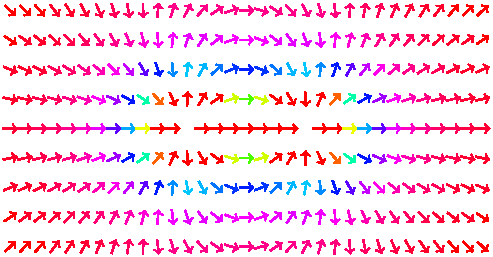
\includegraphics{examples.beamer/field-crop}
	\end{center}
\end{frame}
\mode*

Hopefully, this should be of interest, but mostly as an example of something that is not particularly efficient in Ti\emph{k}Z.
Essentially, the code, in Listing \ref{listing.examples.field}, models the electric field due to several charged particles in 2D space, the resulting graphic uses hue to represent field strength and an arrow to illustrate field direction, as in Figure \ref{figure.examples.fields}.

\begin{figure}[btp]
	\centering
	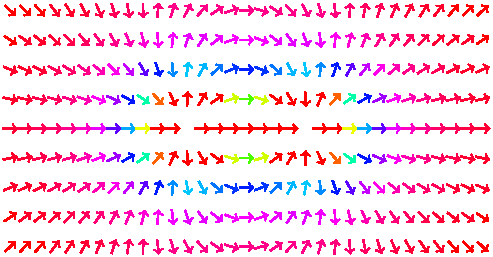
\includegraphics{examples.beamer/field-crop}
	\caption{Computing and illustrating vector fields using TikZ and PGF}
	\label{figure.examples.fields}
\end{figure}

\lstinputlisting[language=TeX, caption={Illustrating a vector field using TikZ and PGF.}, label={listing.examples.field}]{examples.beamer/field}
